\documentclass{standalone}
\usepackage{tikz}
\begin{document}

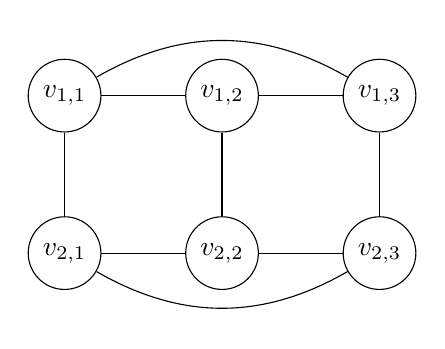
\begin{tikzpicture}[every node/.style={circle, draw, minimum size=8mm}]

% A G_{2,3} graph

\node (11) at (0,0) {$v_{1,1}$};
\node (12) at (2,0) {$v_{1,2}$};
\node (13) at (4,0) {$v_{1,3}$};
\node (21) at (0,-2) {$v_{2,1}$};
\node (22) at (2,-2) {$v_{2,2}$};
\node (23) at (4,-2) {$v_{2,3}$};

% edges

\draw (11) -- (21);
\draw (12) -- (22);
\draw (13) -- (23);
\draw (11) -- (12);
\draw (12) -- (13);
\draw (21) -- (22);
\draw (22) -- (23);
\draw [bend left] (11) to (13);
\draw [bend right] (21) to (23);

\end{tikzpicture}

\end{document}